
\chapter{A new automaton model -- Deterministic Suffix-Reading Automata}
\label{sec:new-automaton-model}

The preceding chapters established that while Deterministic Finite Automata (DFAs) are the canonical model for regular languages, their practical application is often limited by the state-space explosion problem. This has motivated a long-standing search in automata theory for more succinct, yet still deterministic, models of computation.

One prominent approach to achieving conciseness is to allow transitions to be labeled with strings or more complex patterns instead of single symbols. This is seen in models like Deterministic Generalized Automata (DGAs)~\cite{giammarresi1999deterministic} and Deterministic Expression Automata (DEAs)~\cite{DBLP:conf/wia/HanW04}. In a DGA, a transition $q \xrightarrow{\alpha} q'$ is taken from state $q$ only if the remaining input word has the string $\alpha$ as a prefix. The word $\alpha$ is then consumed, and computation continues from state $q'$. This prefix-matching semantic is effective for collapsing linear chains of DFA states into a single transition. However, it is inherently rigid; a DGA cannot ignore or "skip" over intermediate segments of the input stream. This makes it ill-suited for specifying behaviors where an action should be triggered by a specific pattern appearing anywhere in the input, irrespective of what precedes it. DEAs, which use regular expressions, offer more power but come with significant restrictions on the expressions to maintain determinism, ultimately limiting their general applicability.

This chapter introduces a fundamentally different paradigm for string-based automata: `suffix-reading'. Instead of actively consuming prefixes from the remaining input, our model operates on a "wait-and-jump" principle based on the suffixes of the word read so far. The core conceptual shift is from asking, "Does the start of the remaining input match my transition label?" (the DGA approach) to asking, "Does the input processed thus far end with one of my trigger patterns?".

In a Deterministic Suffix-reading Automaton (DSA), a state does not just represent the endpoint of processing a given set of strings, but rather enables a mode of "waiting" for a specific set of patterns to appear. This allows the automaton to passively consume long sequences of irrelevant inputs, only becoming active when a meaningful, pre-defined pattern is detected as a suffix of the history. This approach is designed to more naturally capture the logic of specifications that are "pattern-intensive."

In the sections that follow, we will formalize this intuition. We will provide the complete syntax for DSAs, followed by a rigorous definition of their operational semantics, which resolves ambiguity through novel rules for earliest and longest matching patterns. We will then establish the model's theoretical properties, proving that it retains the full expressive power of DFAs for regular languages and analyzing its potential for providing significantly more succinct specifications.

%marker


We have seen an example of a deterministic suffix automaton in
Figure~\ref{fig:if-else}. A DSA consists of a set of states, and a
finite set of outgoing labels at each state. On an input word $w$, the
DSA finds the earliest prefix which ends with an outgoing label of the
initial state, erases this prefix and goes to the target state of the
transition with the matching label. Now, the DSA processes the rest of
the word from this new state in the same manner. In this section, we
will formally describe the syntax and semantics of DSA.

We start with some more examples. Figure~\ref{fig:example-aab} shows a
DSA for $L_2 = \Sigma^* aab$, the same language as the automata $M_2$
and $H_2$ of Figure~\ref{fig:dfa-dga-examples}. At $q_0$, DSA $\Aa_2$
waits for the first occurrence of $aab$ and as soon as it sees one, it
transitions to $q_3$. Here, it waits for further occurrences of
$aab$. For instance, on the word $abbaabbbaab$, it starts from $q_0$
and reads until $abbaab$ to move to $q_3$. Then, it reads the
remaining $bbaab$ to loop back to $q_3$ and accepts. On a word
$baabaa$, the automaton moves to $q_3$ on $baab$, and continues
reading $aa$, but having nowhere to move, it makes no transition and
rejects the word. Consider another language
$L_3 = \Sigma^*ab\Sigma^*bb$ on the same alphabet $\Sigma$. A similar
machine (as $\Aa_2$) to accept $L_3$ would look like $\Aa_3$ depicted
in Fig.~\ref{fig:example-ab-bb}. For example, on the word $abbbb$, it
would read until $ab$ and move from $q_0$ to $q_1$, read further until
$bb$ and move to $q_2$, then read $b$ and move back to $q_2$ to
accept. We can formally define such machines as automata that
transition on suffixes, or suffix-reading automata.
\begin{figure}
  \centering
  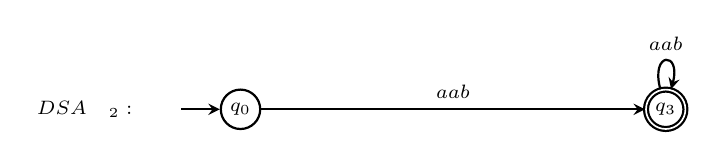
\begin{tikzpicture}[state/.style={circle, draw, thick, inner sep =
      2pt}]
    \begin{scope}[every node/.style={state}]
      \node (0) at (0,0) {\scriptsize $q_0$}; \node [double] (1) at
      (5.4,0) {\scriptsize $q_3$};
    \end{scope}
    \begin{scope}[->, thick, >=stealth, auto]
      \draw (-0.75, 0) to (0); \draw (0) to node {\scriptsize $aab$}
      (1); \draw (1) to [loop above] node {\scriptsize $aab$} (1);
      
    \end{scope}
    
    \node [left] at (-1.25, 0) {\scriptsize $DSA \quad \Aa_2:$};
  \end{tikzpicture}
  \caption{DSA $\Aa_2$ accepts $L_2 = \Sigma^*aab$, with
    $\Sigma = \{a, b\}$.}
  \label{fig:example-aab}
\end{figure}





\begin{definition}[DSA]\label{def:suff-reading-aut}
  A \emph{deterministic suffix-reading automaton (DSA)} $\Aa$ is given by a
  tuple $(Q, \Sigma, q^{init}, \Delta, F)$ where $Q$ is a finite set
  of states, $\Sigma$ is a finite alphabet, $q^{init} \in Q$ is the
  initial state, $\Delta \incl Q \times \Sigma^+ \times Q$ is a finite
  set of transitions, $F \incl Q$ is a set of accepting states.  For a
  state $q \in Q$, we define
  $\out(q) := \{ \a \mid (q, \a, q') \in \Delta \text{ for some } q'
  \in Q \}$ for the set of labels present in transitions out of
  $q$. No state has two outgoing transitions with the same label:
  if $(q, \alpha, q') \in \Delta$ and $(q, \alpha, q'') \in \Delta$,
  then $q' = q''$.
  
  The (total) size $|\Aa|$ of DSA $\Aa$ is defined as the sum of
  the number of states, the number of transitions, and the size
  $|\out(q)|$ for each $q \in Q$, where
  $|\out(q)| := \sum_{\a \in \out(q)} |\a|$.

  
\end{definition}


\begin{figure}[t]
  \centering
  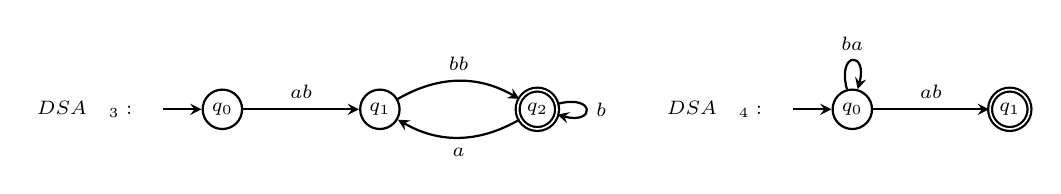
\begin{tikzpicture}[state/.style={circle, draw, thick, inner sep =
      2pt}]
    \begin{scope}[every node/.style={state}]
      \node (0) at (0,0) {\scriptsize $q_0$}; \node (1) at (2,0)
      {\scriptsize $q_1$}; \node [double] (2) at (4,0) {\scriptsize
        $q_2$};
    \end{scope}
    \begin{scope}[->, thick, >=stealth, auto]
      \draw (-0.75, 0) to (0); \draw (0) to node {\scriptsize $ab$ }
      (1); \draw (1) to [bend left=30] node {\scriptsize $bb$} (2);
      \draw (2) to [loop right] node {\scriptsize $b$} (2); \draw (2)
      to [bend left=30] node {\scriptsize $a$} (1);
    \end{scope}
    \node at (-1.75, 0) {\scriptsize $DSA \quad \Aa_3:$};

    \begin{scope}[xshift=8cm]
      \begin{scope}[every node/.style={state}]
        \node (0) at (0,0) {\scriptsize $q_0$}; \node [double] (1) at
        (2,0) {\scriptsize $q_1$};
      \end{scope}
      \begin{scope}[->, thick, >=stealth, auto]
        \draw (-0.75, 0) to (0); \draw (0) to node {\scriptsize $ab$}
        (1); \draw (0) to [loop above] node {\scriptsize $ba$} (0);
      
      \end{scope}

      \node at (-1.75, 0) {\scriptsize $DSA \quad \Aa_4:$};
    \end{scope}
  \end{tikzpicture}
  \caption{$\Aa_3$ accepts $L_3=\Sigma^* ab \Sigma^*bb$ and $\Aa_4$
    accepts $L_4=(b^*ba)^*a^*ab$.}
  \label{fig:example-ab-bb}
\end{figure}

As mentioned earlier, at a state $q$ the automaton waits for a word
that ends with one of its outgoing labels. If more than one label matches,
then the transition with the longest label is taken.  For example, consider the
DSA in Figure~\ref{fig:if-else}. At
state $s_1$ on reading $fghendif$, both the \texttt{if} and
\texttt{endif} transitions match. The longest match is \texttt{endif}
and therefore the DSA moves to $s_0$. This gives a deterministic
behaviour to the DSA. More precisely: at a state $q$, it reads $w$ to
fire $ (q, \a, q') $ if $\a$ is the longest word in $\out(q)$ which is
a suffix of $w$, and no proper prefix of $w$ has any label in
$\out(q)$ as suffix.  We call this a `move' of the DSA. For example,
consider $\Aa_4$ of Figure~\ref{fig:example-ab-bb} as a DSA. Let us
denote $t := (q_0, ab, q_1)$ and $t':= (q_0, ba, q_1)$. We have moves
$(t, ab)$, $(t, aab)$, $(t, aaab)$, and $(t', ba)$, $(t', bba)$,
etc. In order to make a move on $t$, the word should end with $ab$ and
should have neither $ab$ nor $ba$ in any of its proper prefixes.


\begin{definition}\label{def:DSA-moves}
  A \emph{move} of DSA $\Aa$ is a pair $(t, w)$ where
  $t = (q, \a, q') \in \Delta$ is a transition of $\Aa$ and
  $w \in \Sigma^+$ such that
  \begin{itemize}
  \item 
    $\a$ is the longest word in $\out(q)$ which is a suffix of $w$,
    and
  \item 
    no proper prefix of $w$ has a label in $\out(q)$ as
    suffix (no label is a factor of $w$).
  \end{itemize}
  A move $(t, w)$ denotes that at state $q$, transition $t$ gets
  triggered on reading word $w$. We will also write
  $q \xra[\a]{~w~} q'$ for the move $(t, w)$.
\end{definition}


Whether a word is accepted or rejected is determined by a `run' of the
DSA on it. 

\begin{definition}
  A run of $\Aa$ on word $w$, starting from a state $q$, is a sequence
  of moves that consume the word $w$, until a (possibly empty) suffix
  of $w$ remains for which there is no move possible: 
  
  formally, a run
  is a sequence of moves $q_i \xra[\a_i]{~w_i~} q_{i+1}$ for $0\le i\le m$ and $q_m \xra{w_m}$ where $q=q_0$ and $m$ is the index of the last state in the sequence i.e.
  $q = q_0 \xra[\a_0]{~w_0~} q_1 \xra[\a_1]{~w_1~} \cdots
  \xra[\a_{m-1}]{~w_{m-1}~} q_m \xra{w_m}$ such that
  $w=w_0 w_1 \dots w_{m-1} w_m$, and $q_m \xra{w_m}$ denotes that
  there is no move using any outgoing transition from $q_m$ on $w_m$
  or any of its prefixes. 
  
  The run is accepting if $q_m \in F$ and
  $w_m = \e$ (no dangling letters in the end). The language $\Ll(\Aa)$
  of $\Aa$ is the set of all words that have an accepting run starting
  from the initial state $q^{init}$.
\end{definition}

Naturally, the set of words with accepting runs gives the
language of the DSA. Moreover, due to our ``move'' semantics, there is
a unique run for every word.



\section{Comparison with DFA and DGA}
\label{sec:comparison-with-dfa}

Every complete DFA can be seen as an equivalent DSA --- since
$\out(q) = \Sigma$ for every state, the equivalent DSA is forced to
move on each letter, behaving like the DFA that we started off
with. For the DSA-to-DFA direction, we associate a specific DFA to
every DSA, as follows. The idea is to replace transitions of a DSA
with a string-matching-DFA for $\out(q)$ at each
state. Figure~\ref{fig:dsa-to-dfa-eg} gives an example. The
intermediate states correspond to proper prefixes of words in
$\out(q)$.




\begin{definition}[Tracking DFA for a DSA.]\label{def:tracking-dfa}
  For a DSA $\Aa = (Q^\Aa, \Sigma, q_{in}^\Aa, \Delta^\Aa, F^\Aa)$, we
  give a DFA $M_{\Aa}$, called its \emph{tracking DFA}. For
  $q \in Q^\Aa$, let $\outp(q)$ be the set of all prefixes of words in
  $\out(q)$.  States of $M_{\Aa}$ are given by:
  $Q^M = \bigcup_{q \in Q^\Aa} \{ \{ (q, \beta) \mid \beta \in \outp(q)\} \cup
  \{(q,\overline{\epsilon})\} \}$, where $\overline{\epsilon}$ is used as a special symbol to create a copy of each $(q,\epsilon)$. 

  The initial state is $(q^\Aa_{in}, \epsilon)$ and final states are
  $\{ (q, \epsilon) \mid q \in F^\Aa\}$. Transitions are as below: for
  every $q \in Q^\Aa, \beta \in \outp(q), a \in \Sigma$, let $\beta'$ be the
  longest word in $\outp(q)$ s.t $\beta'$ is a suffix of $\beta
  a$. 
  \begin{itemize}
  \item $(q, \beta) \xra{a} (q', \epsilon)$ if $\beta' \in \out(q)$ and  
    $(q,\beta', q') \in \Delta^\Aa$, 
  \item $(q, \beta) \xra{a} (q, \beta')$ if $\beta' \notin \out(q)$ and
    $\beta' \neq \epsilon$,
  \item $(q, \beta) \xra{a} (q,\overline{\epsilon})$ if $\beta' = \epsilon$,
  \item $(q,\overline{\epsilon}) \xra{a} s$, if $(q, \epsilon) \xra{a} s$ according
    to the above (same outgoing transitions).
  \end{itemize}

\end{definition}

\begin{figure}
  \centering
  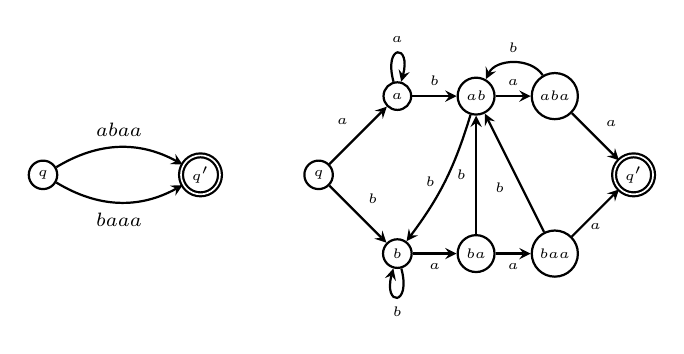
\begin{tikzpicture}[state/.style={circle, draw, thick, inner sep =
      2pt}]
    \begin{scope}[every node/.style={state}]
      \node (0) at (0,0) {\tiny $q$}; \node [double] (1) at (2,0)
      {\tiny $q'$};
    \end{scope}
    \begin{scope}[->, >=stealth, thick, auto]
      \draw (0) to [bend left=30] node {\scriptsize $abaa$} (1); \draw
      (0) to [bend right=30] node [below] {\scriptsize $baaa$} (1);
    \end{scope}

    \begin{scope}[xshift=3.5cm]
      \begin{scope}[every node/.style={state}]
        \node (0) at (0,0) {\tiny $q$}; \node (a) at (1,1) {\tiny
          $a$}; \node (b) at (1,-1) {\tiny $b$}; \node (ab) at (2, 1)
        {\tiny $ab$}; \node (ba) at (2,-1) {\tiny $ba$}; \node (aba)
        at (3, 1) {\tiny $aba$}; \node (baa) at (3,-1) {\tiny $baa$};
        \node [double] (1) at (4, 0) {\tiny $q'$};
      
      \end{scope}
      \begin{scope}[->,>=stealth, thick, auto]
        \draw (0) to node {\tiny $a$} (a); \draw (0) to node {\tiny
          $b$} (b); \draw (a) to node {\tiny $b$} (ab); \draw (b) to
        node [below] {\tiny $a$} (ba); \draw (ab) to node {\tiny $a$}
        (aba); \draw (ba) to node [below] {\tiny $a$} (baa); \draw
        (aba) to node {\tiny $a$} (1); \draw (baa) to node [below]
        {\tiny $a$} (1); \draw (b) to [loop below] node {\tiny $b$}
        (0); \draw (a) to [loop above] node {\tiny $a$} (a); \draw
        (ba) to node {\tiny $b$} (ab); \draw (baa) to node {\tiny $b$}
        (ab); \draw (ab) to [bend left=10] node [left] {\tiny $b$}
        (b); \draw (aba) to [bend right=60] node [above] {\tiny $b$}
        (ab);
      \end{scope}

    \end{scope}

  \end{tikzpicture}
  \caption{A DSA on the left, and the corresponding DFA for matching
    the strings $abaa$ and $baaa$.}
  \label{fig:dsa-to-dfa-eg}
\end{figure}

Intuitively, the tracking DFA implements the transition semantics of
DSAs. Starting at $(q, \e)$, the tracking DFA moves along states
marked with $q$ as long as no label of $\out(q)$ is seen as a
suffix. For all such words, the tracking DFA maintains the longest
word among $\outp(q)$ seen as a suffix so far. For instance, in
Figure~\ref{fig:dsa-to-dfa-eg}, at $q$ on reading word $aab$, the DFA
on the right is in state $ab$ (which is the equivalent of $(q, ab)$ in
the tracking DFA definition).

In the rest of the document, we will make use of the following notation:

\begin{definition}[Notation]
  \label{def:notation}
  
\begin{itemize}
  For two words $w_1, w_2$, we write $w_1 \sfx w_2$ if $w_1$
   is a suffix of $w_2$.
 \item For a set of words $U \incl \Sigma^*$ and $\a, \beta \in \Sigma^*$,
 $\a \lsfx{U} \beta$ if $\a$ is the longest word in $U$ which is a
 suffix of $\beta$, i.e. for all $\a' \in U$ if $\a' \sfx \beta$ then
 $|\a'| \leq |\a|$.


\end{itemize}
\end{definition}

\begin{restatable}{lemma}{trackingDFAEquivalent}
  \label{lem:tracking-dfa-language-equivalent}
  For every DSA $\Aa$, the language $\Ll(\Aa)$ equals the language
  $\Ll(M_\Aa)$ of its tracking DFA.
\end{restatable}

\begin{proof}
  The tracking DFA satisfies the following invariants on every state
  $(q, \epsilon)$: (we make use of notations from
  Definition~\ref{def:notation}) 
  \begin{itemize}
  \item Let $w$ be a word that has no $\a \in \out(q)$ as its
    factor. Then, the run of $w$ starting at $(q, \e)$, remains in
    states of the form $(q, \beta)$ and ends in state $(q, \beta_w)$
    where $\beta_w \lsfx{\outp(q)} w$.
  \item Let $w$ be a word such that $q \xra[\a]{w} q'$ is a move of
    $\Aa$. Then the run of $M_\Aa$ on $w$ starting at $(q, \e)$
    remains in states of the form $(q, \beta)$ and ends in $(q', \e)$.
  \item Let $w$ be a word such that the run of $M_\Aa$ starting at
    $(q, \e)$ remains in states of the form $(q, \beta)$ and ends in a
    state $(q, \beta_w)$. Then $\beta_w \lsfx{\outp(q)} w$.
  \item Let $w$ be a word such that the run of $M_\Aa$ starting at
    $(q, \e)$ ends in $(q', \e)$, and all intermediate states are of
    the form $(q, \beta)$. Then there is a move $q \xra[\a]{w} q'$ in
    $\Aa$ where $\a \lsfx{\out(q)} w$.
  \end{itemize}
  All these invariants can be proved by induction on the length of the
  word $w$ and making use of the way the transitions have been defined
  in the tracking DFA. The first two invariants show that every
  accepting run of $\Aa$ has a corresponding accepting run in $M_\Aa$,
  thereby proving $\Ll(\Aa) \incl \Ll(M_\Aa)$. The next two invariants
  show that every accepting run of $M_\Aa$ corresponds to an accepting
  run of $\Aa$, thereby showing $\Ll(M_\Aa) \incl \Ll(\Aa)$.
\end{proof}


Lemma~\ref{lem:tracking-dfa-language-equivalent} and the fact that
every complete DFA is also a DSA, prove that DSAs recognize regular
languages. We will now compare succinctness of DSA wrt DFA and DGA,
starting with a family of languages for which DSAs are concise.




\begin{restatable}{lemma}{dsaSmall}
  \label{lem:dsa-small}
  Let $\Sigma = \{a_1, a_2, \dots, a_n\}$ for some $n \ge 1$. Consider
  the language $L_n = \Sigma^* a_1 a_2 \dots a_n$. There is a DSA for
  this language with size $(4 + 2 |\Sigma|)$.  Any trim DFA for $L_n$ has size at
  least ${|\Sigma|}^2$. (Note: size is counted as the sum of the number of
  states, edges and length of edge labels, in all the automata) 
\end{restatable}

\begin{proof}
  Consider the DSA with states $q_0, q_1$ and transitions
  $q_0 \xra{a_1 \dots a_n} q_1$, $q_1 \xra{a_1 \dots a_n} q_1$, with
  $q_0$ the initial state and $q_1$ the accepting state. This DSA
  accepts $L_n$.

  For any pair $a_1 a_2 \dots a_i$ and $a_1 a_2 \dots a_j$ with
  $i \neq j$, there is a distinguishing suffix:
  $a_1 a_2 \dots a_i \cdot a_{i+1} \dots a_n \in L_n$, but
  $a_1 a_2 \dots a_j \cdot  a_{i+1} \dots a_n \notin
  L_n$. Therefore, the strings $a_1$, $a_1a_2$, $\dots$,
  $a_1 \dots a_n$ go to different states in the canonical DFA. This
  shows there are at least $n$ states in the minimal DFA. Now, from
  $a_1 a_2 \dots a_j$, there is a transition of every letter: clearly,
  there needs to be a transition on $a_{j+1}$; if there is no
  transition on, say $a_\ell \neq a_{j+1}$, then the word
  $a_1 a_2 \dots a_j a_\ell a_1 a_2 \dots a_n$ will be rejected. A
  contradiction. Hence, there are $n$ transitions from each state.
\end{proof}

We make a remark about DGAs for the language family in
Lemma~\ref{lem:dsa-small}. Notice that suppressing superfluous states
of the minimal DFA leads to a strict increase in the label length,
which only strictly increases the (total) size. For instance, suppose
$q_1 \xra{a_2} q_2 \xra{a_3} q_3$ is a sequence of transitions in the
minimal DFA for $L_n$. There are additional transitions
$q_2 \xra{a_1} q_1$ and $q_2 \xra{\Sigma \setminus \{a_1, a_3\}} q_0$
(where $q_0$ is the initial state). Suppressing $q_2$ leads to edges
with labels $a_2a_3$, $a_2a_1$, $a_2 c$ for each
$c \in \Sigma \setminus \{a_1, a_3\}$. Notice that $a_2$ gets copied
$|\Sigma|$ many times. Therefore suppressing states from the minimal
DFA is not helpful in getting a smaller DGA. However, using this
argument, we cannot conclude that the minimal DGA has size at least
$n^2$. Since a characterization of minimality of DGAs in terms of
total size is not known, we leave it at this remark.


We now state the final result of this section, which summarizes the
size comparison between DSAs, DFAs, DGAs. For the comparison to DFAs,
we use the fact that every DSA of size $k$ can be converted to its
tracking DFA, which has atmost $2k$ states. Therefore, size of the
tracking DFA is
bounded by $2k$ (states) $ + 2k \cdot |\Sigma|$ (edges)
$ + 2k \cdot |\Sigma|$ (label length), which comes to
$2k ( 1+ 2|\Sigma|)$.

For a regular language $L$, let
  $n_F^{cmp}(L), n_F^{trim}(L), n_G^{trim}(L), n_S(L)$ denote the size of the
  minimal complete DFA, minimal trim DFA, minimal trim DGA and minimal
  DSA respectively, where size is counted as the sum of the number of
  states, edges and length of edge labels, in all the automata. 

\begin{restatable}{theorem}{comparison}\label{thm:comparing-dsa-with-dfa-dga}
  We have:
  \begin{enumerate}
  \item For all $L$, we have $\dfrac{n_F^{cmp}(L)}{2 (1 + 2|\Sigma|)} \le n_S(L) \le n_F^{cmp}(L)$
  \item %no relation between $n_S$ and $n_F^{trim}, n_G^{trim}$: 
  There is a language for which $n_S(L)$ is the smallest, and another
    language for which $n_S(L)$ is the largest of the three.
  \end{enumerate}

\end{restatable}

\begin{proof}
  A complete DFA can be seen as a DSA accepting the same
  language. This gives us $n_S(L) \le n_F^{cmp}(L)$. For the inequality
  $\dfrac{n_F^{cmp}(L)}{2 (1 + 2|\Sigma|)} \le n_S(L)$, we show that the
  tracking DFA (Definition~\ref{def:tracking-dfa}) of a DSA has size
  at most $n_S(L) \cdot 2 (1 + 2|\Sigma|)$. The number of states of the
  tracking DFA is atmost $2 n_S(L)$ (recall that $n_S(L)$ denotes the total size of the DSA, which includes the label lengths). For each state there are $\Sigma$
  transitions. Therefore, total size is $2n_S(L)$ (states) + $2n_S(L) \cdot
 |\Sigma|$ (edges) + $2 n_S(L) \cdot |\Sigma|$ (label lengths), which equals
 $2 n_S(L) (1 + 2 |\Sigma|)$.

 For the second part of the proof, Lemma~\ref{lem:dsa-small} gives an
 example where $n_S(L)$ is the smallest. For the other direction,
 consider the language $L_1 = (ab)^*$. A trim DFA for this language has two
 states $q_0, q_1$ (with $q_0$ accepting), and two transitions $q_0 \xra{a} q_1$, and $q_1
 \xra{b} q_0$. Therefore $n_F^{trim}(L_1) \le 2 + 2 + 2 = 6$. A trim DGA
 for this language is $q_0 \xra{ab} q_0$. Therefore $n_G^{trim}(L_1) \le 2
 + 1 + 2 = 5$. We first claim that any DSA for this language needs to
 maintain the following information: (1) the initial state which is
 accepting, as $\e$ is in the 
 language; (2) there is a path from the initial state on
 $ab$ to an accepting state (otherwise $ab$ will not be accepted); (3)
 on reading $aa$ or $b$ from the initial state, the DSA has to make 
 some transitions and go to a sink state, which is a non-accepting state
 --- otherwise,  the words $aab$ or $bab$ will get accepted. This shows that any
 DSA has at least two states, at least three transitions, and ${ab}$, $b$ and ${aa}$ split across some transition labels. This gives either: $n_S(L_1) \ge 2 + 2 + 4 = 8$ for the DSA with two states and $\xra{ab}$, $\xra{b}$ and $\xra{aa}$ as transitions, which is bigger than
 the corresponding trim DFA and DGA, or the min DFA viewed as DSA, with 3 states, and transitions on each of $a$ and $b$ from each of the states giving $n_S \ge3+6+6 = 15$
\end{proof}



%%% Local Variables:
%%% mode: latex
%%% TeX-master: "dsa-main"
%%% End:

This chapter has laid the complete theoretical groundwork for Deterministic Suffix-reading Automata. We began with a formal syntax in \textbf{Definition \ref{def:suff-reading-aut}}, introducing not only the structure of the automaton but also the \textbf{total-size} metric, a more faithful measure of descriptive complexity for models with string-based transition labels. The core idea of the model was detailed through its unique operational semantics, where we established how a DSA defines a deterministic run by adhering to two principles: acting on the \textbf{earliest} occurrence of a recognizable pattern, and in cases of ambiguity, choosing the transition corresponding to the \textbf{longest matching suffix}.

A central result of this chapter was the proof that DSAs recognize exactly the class of \textbf{regular languages}. This was established constructively through the \textbf{tracking DFA} construction (Definition 3.4), a method for converting any DSA into an equivalent, standard DFA. This result firmly grounds our new model within classical automata theory, ensuring it is a new representation for a well-understood class of languages, rather than an extension into non-regular territory. Finally, we quantified the primary motivation for this new model: \textbf{succinctness}. By analyzing a family of languages ($L_n = \Sigma^* a_1 a_2 \dots a_n$), we formally demonstrated that a DSA can be exponentially more concise in total size than the minimal DFA for the same language, highlighting its potential for modeling pattern-intensive specifications.

With the model's theoretical properties and potential benefits now established, the focus naturally shifts from the abstract to the constructive. A formal model is only as useful as our ability to create instances of it for practical problems. This leads to the central question that will drive the next chapter: Given a regular language, typically represented by a DFA, how can we derive a language-equivalent and concise DSA? We will answer this by presenting a systematic DFA-to-DSA conversion procedure. This investigation will, in turn, unveil some counter-intuitive challenges of DSA minimization, revealing fundamental ways in which suffix-reading automata differ from their classical counterparts.